\section{eo\-Init\-Fixed\-Length$<$ EOT $>$ Class Template Reference}
\label{classeo_init_fixed_length}\index{eoInitFixedLength@{eoInitFixedLength}}
Initializer for fixed length representations with a single type.  


{\tt \#include $<$eo\-Init.h$>$}

Inheritance diagram for eo\-Init\-Fixed\-Length$<$ EOT $>$::\begin{figure}[H]
\begin{center}
\leavevmode
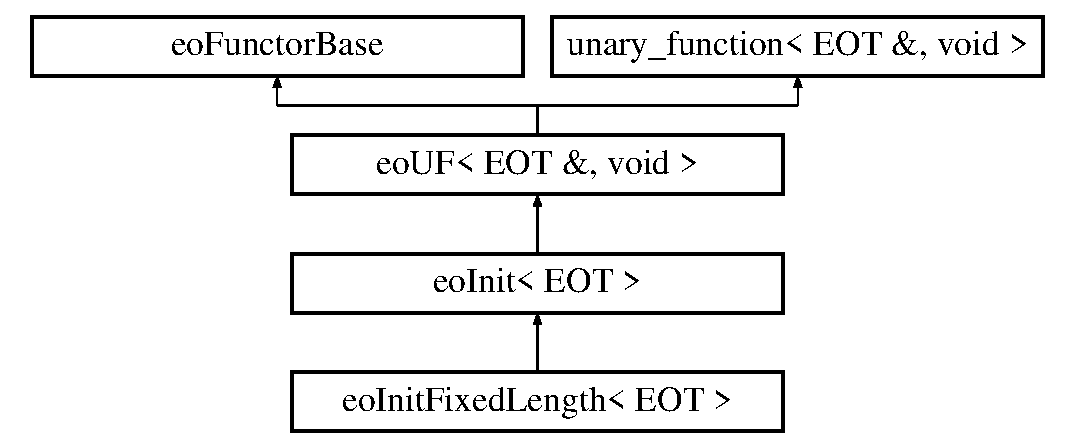
\includegraphics[height=4cm]{classeo_init_fixed_length}
\end{center}
\end{figure}
\subsection*{Public Types}
\begin{CompactItemize}
\item 
typedef EOT::Atom\-Type {\bf Atom\-Type}\label{classeo_init_fixed_length_w0}

\end{CompactItemize}
\subsection*{Public Member Functions}
\begin{CompactItemize}
\item 
{\bf eo\-Init\-Fixed\-Length} (unsigned \_\-combien, {\bf eo\-Rnd\-Generator}$<$ Atom\-Type $>$ \&\_\-generator)\label{classeo_init_fixed_length_a0}

\item 
virtual void {\bf operator()} ({\bf EOT} \&chrom)\label{classeo_init_fixed_length_a1}

\begin{CompactList}\small\item\em The pure virtual function that needs to be implemented by the subclass. \item\end{CompactList}\end{CompactItemize}
\subsection*{Private Attributes}
\begin{CompactItemize}
\item 
unsigned {\bf combien}\label{classeo_init_fixed_length_r0}

\item 
{\bf eo\-STLF}$<$ Atom\-Type $>$ {\bf generator}\label{classeo_init_fixed_length_r1}

\begin{CompactList}\small\item\em generic wrapper for eo\-Functor (s), to make them have the function-pointer style copy semantics \item\end{CompactList}\end{CompactItemize}


\subsection{Detailed Description}
\subsubsection*{template$<$class EOT$>$ class eo\-Init\-Fixed\-Length$<$ EOT $>$}

Initializer for fixed length representations with a single type. 



Definition at line 81 of file eo\-Init.h.

The documentation for this class was generated from the following file:\begin{CompactItemize}
\item 
eo\-Init.h\end{CompactItemize}
